%===============================================================================
% LaTeX sjabloon voor de bachelorproef toegepaste informatica aan HOGENT
% Meer info op https://github.com/HoGentTIN/latex-hogent-report
%===============================================================================

\documentclass[dutch,dit,thesis]{hogentreport}

% - If necessary, replace the option `dit`' with your own department!
%   Valid entries are dbo, dbt, dgz, dit, dlo, dog, dsa, soa
% - If you write your thesis in English (remark: only possible after getting
%   explicit approval!), remove the option "dutch," or replace with "english".

\usepackage{lipsum} % For blind text, can be removed after adding actual content

%% Glossaries and acronyms
\usepackage[acronym,nomain,toc]{glossaries}

\makeglossaries

\newacronym{poc}{PoC}{Proof-of-Concept}
\newacronym{uiux}{UI/UX}{User Interface / User Experience}
\newacronym{icd}{ICD}{International Classifiction of Diseases}
\newacronym{who}{WHO}{Wereldhandelsorganisatie}
\newacronym{qlc}{QLC}{Quarter Life Crisis}
\newacronym{clt}{CLT}{Cognitive Load Theory}
\newacronym{dcl}{DCL}{Digital Cognitive Load}
\newacronym{io}{IO}{Information Overload}
\newacronym{ifomo}{IFoMO}{Informational Fear of Missing Out}

%% Pictures to include in the text can be put in the graphics/ folder
\graphicspath{{../graphics/}}

%% For source code highlighting, requires pygments to be installed
%% Compile with the -shell-escape flag!
%% \usepackage[chapter]{minted}
%% If you compile with the make_thesis.{bat,sh} script, use the following
%% import instead:
\usepackage[chapter,outputdir=../output]{minted}
\usemintedstyle{solarized-light}

%% Formatting for minted environments.
\setminted{%
    autogobble,
    frame=lines,
    breaklines,
    linenos,
    tabsize=4
}

%% Ensure the list of listings is in the table of contents
\renewcommand\listoflistingscaption{%
    \IfLanguageName{dutch}{Lijst van codefragmenten}{List of listings}
}
\renewcommand\listingscaption{%
    \IfLanguageName{dutch}{Codefragment}{Listing}
}
\renewcommand*\listoflistings{%
    \cleardoublepage\phantomsection\addcontentsline{toc}{chapter}{\listoflistingscaption}%
    \listof{listing}{\listoflistingscaption}%
}

% Other packages not already included can be imported here

%%---------- Document metadata -------------------------------------------------
\author{Britt Emanuel}
\supervisor{Mevr. C. De Leenheer}
\cosupervisor{Mevr. N. Jacobs, Mevr. K. Van den Broeck}
\title[Een vergelijkende analyse en proof-of-concept]%
    {Burn-outpreventie bij Vlaamse twintigers: een vergelijkende studie van bestaande apps en de vertaling naar ontwerpprincipes voor een stressreducerende applicatie}
\academicyear{\advance\year by -1 \the\year--\advance\year by 1 \the\year}
\examperiod{1}
\degreesought{\IfLanguageName{dutch}{Professionele bachelor in de toegepaste informatica}{Bachelor of applied computer science}}
\partialthesis{false} %% To display 'in partial fulfilment'
%\institution{Internshipcompany BVBA.}

%% Add global exceptions to the hyphenation here
\hyphenation{back-slash}

%% The bibliography (style and settings are  found in hogentthesis.cls)
\addbibresource{bachproef.bib}            %% Bibliography file
\addbibresource{../voorstel/voorstel.bib} %% Bibliography research proposal
\defbibheading{bibempty}{}

%% Prevent empty pages for right-handed chapter starts in twoside mode
\renewcommand{\cleardoublepage}{\clearpage}

\renewcommand{\arraystretch}{1.2}

%% Content starts here.
\begin{document}

%---------- Front matter -------------------------------------------------------

\frontmatter

\hypersetup{pageanchor=false} %% Disable page numbering references
%% Render a Dutch outer title page if the main language is English
\IfLanguageName{english}{%
    %% If necessary, information can be changed here
    \degreesought{Professionele Bachelor toegepaste informatica}%
    \begin{otherlanguage}{dutch}%
       \maketitle%
    \end{otherlanguage}%
}{}

%% Generates title page content
\maketitle
\hypersetup{pageanchor=true}

%%=============================================================================
%% Voorwoord
%%=============================================================================

\chapter*{\IfLanguageName{dutch}{Woord vooraf}{Preface}}%
\label{ch:voorwoord}

%% TODO:
%% Het voorwoord is het enige deel van de bachelorproef waar je vanuit je
%% eigen standpunt (``ik-vorm'') mag schrijven. Je kan hier bv. motiveren
%% waarom jij het onderwerp wil bespreken.
%% Vergeet ook niet te bedanken wie je geholpen/gesteund/... heeft

In deze bachelorproef onderzoek ik hoe apps voor stress- en burn-outpreventie het mentale welzijn van Vlaamse twintigers kunnen ondersteunen. Dit onderzoek vormt het sluitstuk van mijn opleiding toegepaste informatica, waarna ik hoop af te studeren.

\vspace{1em}

De keuze voor dit onderwerp kwam niet zomaar tot stand. Tijdens de COVID-19-pandemie, gedurende mijn vorige opleiding, merkte ik hoe een hoge werkdruk en te weinig rust hun tol konden eisen. Ik ging daarom zelf op zoek naar digitale toepassingen die konden helpen om meer rust te vinden. Helaas boden deze apps mij niet de ondersteuning die ik ervan verwachtte, waardoor ik ze al snel weer links liet liggen. Deze ervaring deed mij nadenken over hoe zulke toepassingen beter kunnen worden ontworpen. Tijdens deze bachelor ontdekte ik dat mentale gezondheidsapps sterk zijn gegroeid sinds de pandemie, terwijl stress- en burn-outklachten bij jongvolwassenen bleven toenemen. Vanuit die vaststelling ontstond het idee voor deze bachelorproef: onderzoeken waar bestaande toepassingen tekortschieten en deze inzichten vertalen naar richtlijnen voor meer stressreducerende mentale gezondheidsapps.

\vspace{1em}

Het uitvoeren van dit onderzoek was intensief maar bijzonder leerrijk. De combinatie van literatuuronderzoek, requirementsanalyse, mock-ups en de implementatie van de \acrshort{poc} bracht verschillende uitdagingen met zich mee. Niet alle ideeën konden binnen de beschikbare tijd volledig worden uitgewerkt. De literatuurstudie deed mij bovendien inzien hoe belangrijk psychologische basisbehoeften zoals autonomie, competentie en verbondenheid zijn bij het ontwerpen van digitale toepassingen. Dit verbreedde mijn kijk op softwareontwikkeling en maakte de psychologische invalshoek van het onderzoek voor mij bijzonder waardevol. Dankzij mijn copromotor kon ik hierbij rekenen op waardevolle begeleiding en inzichten vanuit de psychologie.

\vspace{1em}

Daarvoor wil ik mijn copromotor, mevrouw K. Van den Broeck, graag bedanken. Ook mijn promotor, mevrouw C. De Leenheer, wil ik bedanken voor haar feedback en begeleiding gedurende het volledige traject. Daarnaast bedank ik meneer T. Parmentier om tijdelijk als vervangende promotor in te vallen. Ten slotte wil ik mijn ouders, mijn zus A. Emanuel en mijn vriend M. Dhondt bedanken voor hun voortdurende steun, motivatie en aanmoediging tijdens het schrijven van deze bachelorproef. Dankzij hen stond ik er tijdens dit traject nooit alleen voor.
%%=============================================================================
%% Samenvatting
%%=============================================================================

% TODO: De "abstract" of samenvatting is een kernachtige (~ 1 blz. voor een
% thesis) synthese van het document.
%
% Een goede abstract biedt een kernachtig antwoord op volgende vragen:
%
% 1. Waarover gaat de bachelorproef?
% 2. Waarom heb je er over geschreven?
% 3. Hoe heb je het onderzoek uitgevoerd?
% 4. Wat waren de resultaten? Wat blijkt uit je onderzoek?
% 5. Wat betekenen je resultaten? Wat is de relevantie voor het werkveld?
%
% Daarom bestaat een abstract uit volgende componenten:
%
% - inleiding + kaderen thema
% - probleemstelling
% - (centrale) onderzoeksvraag
% - onderzoeksdoelstelling
% - methodologie
% - resultaten (beperk tot de belangrijkste, relevant voor de onderzoeksvraag)
% - conclusies, aanbevelingen, beperkingen
%
% LET OP! Een samenvatting is GEEN voorwoord!

%%---------- Nederlandse samenvatting -----------------------------------------
%
% TODO: Als je je bachelorproef in het Engels schrijft, moet je eerst een
% Nederlandse samenvatting invoegen. Haal daarvoor onderstaande code uit
% commentaar.
% Wie zijn bachelorproef in het Nederlands schrijft, kan dit negeren, de inhoud
% wordt niet in het document ingevoegd.

\IfLanguageName{english}{%
\selectlanguage{dutch}
\chapter*{Samenvatting}
\lipsum[1-4]
\selectlanguage{english}
}{}

%%---------- Samenvatting -----------------------------------------------------
% De samenvatting in de hoofdtaal van het document

\chapter*{\IfLanguageName{dutch}{Samenvatting}{Abstract}}

In deze bachelorproef wordt onderzocht hoe apps voor stress- en burn-outpreventie het mentale welzijn van Vlaamse twintigers kunnen ondersteunen. Deze doelgroep wordt steeds sterker blootgesteld aan prestatiedruk, sociale verwachtingen en permanente digitale connectiviteit. Tegelijkertijd nam in België tussen 2018 en 2023 het aantal personen jonger dan 30 jaar dat langdurig arbeidsongeschikt is door burn-out met 107\% toe. Hoewel het aanbod aan digitale toepassingen voor mentaal welzijn sterk is gegroeid, blijven vragen bestaan over hun doelgroepgerichtheid, gebruiksvriendelijkheid en mogelijke cognitieve belasting.

\vspace{1em}

Het onderzoek startte met een literatuurstudie naar stress en burn-out bij twintigers, digitale mentale gezondheidsinterventies, preventiestrategieën, digitalisering en cognitieve belasting, en \acrshort{ui}/\acrshort{ux}-ontwerp. Op basis hiervan en van een interview werden functionele en niet-functionele requirements opgesteld volgens de MoSCoW-methode. Daarnaast werden ontwerpprincipes geformuleerd die beschrijven hoe digitale toepassingen mentale rust kunnen bevorderen en cognitieve belasting kunnen beperken. Deze requirements vormden de basis voor een vergelijkende analyse van bestaande mentale gezondheidsapps. Vijf geselecteerde toepassingen werden geëvalueerd aan de hand van de opgestelde ontwerpprincipes. Hieruit werden relevante functionaliteiten en zowel sterke als minder effectieve ontwerpkeuzes geïdentificeerd. Op basis van deze inzichten werd een cross-platform \acrshort{poc} ontwikkeld met onder meer gepersonaliseerde onboarding, een toolkit met oefeningen, dagboek- en reflectiefuncties, psycho-educatieve content en instelbare notificaties en voorkeuren.

\vspace{1em}

Uit het onderzoek blijkt dat een stressreducerende applicatie niet alleen moet focussen op de aangeboden interventies, maar ook op de manier waarop deze worden aangeboden. Belangrijke uitgangspunten zijn personalisatie, een overzichtelijke interface, beperkte informatie, digitale onderbrekingen, en het vermijden van mechanismen die extra prestatiedruk veroorzaken. Zo wordt aanbevolen om notificaties instelbaar te maken, informatie stapsgewijs aan te bieden, één primaire taak per scherm te hanteren en gamification zoals streaks en rankings te vermijden.

\vspace{1em}

De \acrshort{poc} werd ten slotte heuristisch geëvalueerd aan de hand van de eerder opgestelde requirements en ontwerpprincipes. De resultaten tonen aan dat deze principes bruikbaar zijn als praktisch kader voor het ontwerpen en beoordelen van stressreducerende digitale toepassingen. 

\vspace{1em}

Het onderzoek kent echter beperkingen, waaronder het ontbreken van een evaluatie met de uiteindelijke doelgroep van de app. Er kan daarom niet worden geconcludeerd dat de toepassing daadwerkelijk stress of burn-out vermindert. Verder onderzoek met Vlaamse twintigers is nodig om zowel de ontwerpprincipes als de \acrlong{poc} empirisch te valideren.


%---------- Inhoud, lijst figuren, ... -----------------------------------------

\tableofcontents

% In a list of figures, the complete caption will be included. To prevent this,
% ALWAYS add a short description in the caption!
%
%  \caption[short description]{elaborate description}
%
% If you do, only the short description will be used in the list of figures

\listoffigures

% If you included tables and/or source code listings, uncomment the appropriate
% lines.
\listoftables

\listoflistings

% Als je een lijst van afkortingen of termen wil toevoegen, dan hoort die
% hier thuis. Gebruik bijvoorbeeld de ``glossaries'' package.
% https://www.overleaf.com/learn/latex/Glossaries
\printglossary[title=Acroniemen, toctitle=Acroniemen]

%---------- Kern ---------------------------------------------------------------

\mainmatter{}

% De eerste hoofdstukken van een bachelorproef zijn meestal een inleiding op
% het onderwerp, literatuurstudie en verantwoording methodologie.
% Aarzel niet om een meer beschrijvende titel aan deze hoofdstukken te geven of
% om bijvoorbeeld de inleiding en/of stand van zaken over meerdere hoofdstukken
% te verspreiden!

%%=============================================================================
%% Inleiding
%%=============================================================================

\chapter{\IfLanguageName{dutch}{Inleiding}{Introduction}}%
\label{ch:inleiding}

Burn-outs: een welbekend fenomeen en een steeds groter wordende maatschappelijke problematiek. In het dagelijkse leven belandt men als het ware in een vrij repetitief ritme bestaande uit werk, huishoudelijke taken en beperkte ontspanningsmomenten. Op het eerste gezicht lijkt deze routine vrij onschuldig en normaal. Echter, wanneer dit patroon zich dag na dag herhaalt zonder voldoende balans in het werk en privéleven, kan het bijdragen aan chronische stress en uitputting. 

\vspace{1em}

Wat voor een lange tijd voornamelijk geassocieerd werd met ervaren werknemers in veeleisende functies, blijkt vandaag echter een fenomeen dat zich niet beperkt tot één specifieke leeftijdscategorie. Een burn-out kan in principe zich op elke leeftijd manifesteren. Toch wijzen recente cijfers erop dat vooral jongvolwassenen steeds vaker getroffen worden \autocite{RIZIV2023_invaliditeit_burnout}. Door belangrijke persoonlijke en professionele keuzes alsook de onzekerheden die eigen zijn aan deze levensfase, kampen ze steeds vaker met vragen over hun identiteit, toekomst, capaciteiten en doelen in het leven. Hierdoor is mentale gezondheid één van de meest urgente maatschappelijke uitdagingen voor deze generatie.

\vspace{1em}

Om dit probleem onder handen te nemen hebben verscheidene software- en productontwikkelaars een poging gewaagd tot het ontwikkelen van toepassingen die beogen stress en burn-out te verminderen, wat heeft geleid tot een explosieve groei van mentale welzijn-apps. De aanhoudende stijging van burn-outgevallen suggereren echter dat deze apps tot op heden slechts een beperkter effect hebben. Dit roept de vraag op hoe dergelijke toepassingen kunnen worden verbeterd en succesvol kunnen worden ingezet zodat ze jongvolwassenen effectiever ondersteunen bij het omgaan met de dagelijkse druk en de onzekerheden die onlosmakelijk verbonden zijn aan hun levensfase.

\section{\IfLanguageName{dutch}{Probleemstelling}{Problem Statement}}%
\label{sec:probleemstelling}

\vspace{1em}

Jongvolwassenen, en in het bijzonder Vlaamse twintigers, ervaren een steeds meer toenemende druk door persoonlijke, professionele en sociale uitdagingen. Hun semi-permanente digitale aanwezigheid bemoeilijkt het vinden van een goede werk-privébalans, met een verhoogd risico op stress en burn-out als gevolg. Tegelijkertijd kampen psychologen en andere hulpverleners die deze doelgroep begeleiden met lange wachttijden, volle agenda’s en soms zelfs een patiëntenstop, waardoor tijdige begeleiding voor deze jongvolwassenen steeds moeilijker wordt. 

\vspace{1em}

Digitale toepassingen zoals mentaal welzijn-apps kunnen in dit kader een nuttige rol spelen door extra ondersteuning te bieden, zowel tijdens deze wachttijd als gedurende een mogelijke behandeling. Uit onderzoek blijkt echter dat het effect van de huidige apps vaak beperkt blijft, wat vragen oproept over hun effectiviteit, doelgroepgerichtheid en gebruiksvriendelijkheid. Het analyseren van deze gebreken en het ontwikkelen van een \acrlong{poc} kunnen daarom bijdragen aan een beter afgestemde digitale ondersteuning, die Vlaamse twintigers effectief helpt bij stress- en burn-outpreventie, zorgprofessionals ondersteunt in hun begeleiding en tegelijkertijd hun overvolle agenda verlicht, met een positieve impact op het algemene welzijn van de maatschappij.

\vspace{1em}

\section{\IfLanguageName{dutch}{Onderzoeksvraag}{Research question}}%
\label{sec:onderzoeksvraag}

\subsection{Hoofdonderzoeksvraag}
\label{subsec:hoofdonderzoeksvraag}

\vspace{1em}

In het kader van dit onderzoek en het kunnen uitwerken van een \acrshort{poc}, werd volgende onderzoeksvraag geformuleerd: “Hoe kunnen apps voor stress- en burn-outpreventie het mentale welzijn van Vlaamse twintigers verbeteren, door middel van inzichten uit een analyse van bestaande apps te vertalen naar concrete ontwerpprincipes en functionaliteiten voor een proof-of-concept app?”.

\subsection{Deelvragen}
\label{subsec:deelvragen}

\vspace{1em}

Om de complexe en uitgebreide onderzoeksvraag zo goed mogelijk te beantwoorden werd de hoofdvraag opgedeeld in enkele deelvragen:

\vspace{1em}
\vspace{1em}

\textbf{Deelvragen probleemdomein:}

\begin{itemize}
    \item Welke categorieën bestaan er onder Belgische twintigers en wat zijn hun individuele specifieke noden op vlak van mentale gezondheid?
    \item Hoe beïnvloeden persoonlijke en externe factoren \textit{(werk-, studie- en sociale druk)} de gebruikerservaring van digitale toepassingen, en welke functies en ondersteuning verwachten de verschillende subgroepen?
    \item Welke functies en ontwerpprincipes worden momenteel gebruikt in apps voor mentaal welzijn, en hoe effectief zijn deze?
    \item Welke \acrshort{ui}/\acrshort{ux}-elementen dragen bij aan mentale rust en welke verhogen juist cognitieve belasting?
    \item Waar falen bestaande apps in het ondersteunen van mentale gezondheid en het verminderen van stress of burn-out?
    \item Welke succesvolle ontwerpprincipes zijn herbruikbaar voor andere digitale toepassingen?
    \item Welke initiatieven, buiten apps, ondersteunen het mentale welzijn van twintigers, en welke best practices uit deze initiatieven kunnen worden vertaald naar digitale toepassingen?
\end{itemize}

\vspace{1em}

\textbf{Deelvragen oplossingsdomein:}

\begin{itemize}
    \item Welke functionele en niet-functionele vereisten zijn essentieel voor een app die stress en burn-out bij twintigers helpt voorkomen?
    \item Hoe kan de interface van een app ontworpen worden om mentale rust te bevorderen en cognitieve belasting te minimaliseren?
    \item Hoe kunnen meldingen en gamification zodanig worden ingezet dat ze ondersteunen zonder cognitief te overweldigen?
    \item Welke generieke ontwerpprincipes en functionaliteiten kunnen worden toegepast op andere digitale toepassingen voor mentale gezondheid?
    \item Hoe kunnen deze richtlijnen praktisch geïmplementeerd worden in andere apps?
\end{itemize}

\vspace{1em}

\section{\IfLanguageName{dutch}{Onderzoeksdoelstelling}{Research objective}}%
\label{sec:onderzoeksdoelstelling}

\vspace{1em}

Het beoogde resultaat van deze bachelorproef is het ontwikkelen van een \acrshort{poc}-app die wetenschappelijk onderbouwde technieken en interfaces implementeert om zo stress- en burn-outpreventie bij Vlaamse twintigers te ondersteunen. Daarnaast is het doel om uit het onderzoek een lijst aan concrete richtlijnen en herbruikbare ontwerpprincipes op te stellen welke geïmplementeerd kunnen worden in andere digitale toepassingen gericht op mentale gezondheid.

\vspace{1em}

Om dit te bereiken zal het probleemdomein eerst concreet in kaart worden gebracht via een literatuurstudie en interviews, waarna functionele en niet-functionel requirements worden geformuleerd om te kunnen gebruiken in een vergelijkende studie van apps, websites en andere concepten. Met deze inzichten, richtlijnen en ontwerpprincipes wordt een \acrshort{poc}-app ontwikkeld.

\vspace{1em}

Het onderzoek wordt als succesvol beschouwd wanneer de app aansluit bij de behoeften van de doelgroep, mentale rust bevordert en de geïmplementeerde componenten effectief en correct functioneren volgens de vastgestelde requirements.

\section{\IfLanguageName{dutch}{Opzet van deze bachelorproef}{Structure of this bachelor thesis}}%
\label{sec:opzet-bachelorproef}

\vspace{1em}

% Het is gebruikelijk aan het einde van de inleiding een overzicht te
% geven van de opbouw van de rest van de tekst. Deze sectie bevat al een aanzet
% die je kan aanvullen/aanpassen in functie van je eigen tekst.

De rest van deze bachelorproef is als volgt opgebouwd:

In Hoofdstuk~\ref{ch:stand-van-zaken} wordt een overzicht gegeven van de stand van zaken binnen het onderzoeksdomein, op basis van een literatuurstudie.

In Hoofdstuk~\ref{ch:methodologie} wordt de methodologie toegelicht en worden de gebruikte onderzoekstechnieken besproken om een antwoord te kunnen formuleren op de onderzoeksvragen.

% TODO: Vul hier aan voor je eigen hoofstukken, één of twee zinnen per hoofdstuk

In Hoofdstuk~\ref{ch:conclusie}, tenslotte, wordt de conclusie gegeven en een antwoord geformuleerd op de onderzoeksvragen. Daarbij wordt ook een aanzet gegeven voor toekomstig onderzoek binnen dit domein.
\chapter{\IfLanguageName{dutch}{Stand van zaken}{State of the art}}%
\label{ch:stand-van-zaken}

% Tip: Begin elk hoofdstuk met een paragraaf inleiding die beschrijft hoe
% dit hoofdstuk past binnen het geheel van de bachelorproef. Geef in het
% bijzonder aan wat de link is met het vorige en volgende hoofdstuk.

% Pas na deze inleidende paragraaf komt de eerste sectiehoofding.

% Commentaar = ctrl + t

%Dit hoofdstuk bevat je literatuurstudie. De inhoud gaat verder op de inleiding, maar zal het onderwerp van de bachelorproef *diepgaand* uitspitten. De bedoeling is dat de lezer na lezing van dit hoofdstuk helemaal op de hoogte is van de huidige stand van zaken (state-of-the-art) in het onderzoeksdomein. Iemand die niet vertrouwd is met het onderwerp, weet nu voldoende om de rest van het verhaal te kunnen volgen, zonder dat die er nog andere informatie moet over opzoeken \autocite{Pollefliet2011}.
%
%Je verwijst bij elke bewering die je doet, vakterm die je introduceert, enz.\ naar je bronnen. In \LaTeX{} kan dat met het commando \texttt{$\backslash${textcite\{\}}} of \texttt{$\backslash${autocite\{\}}}. Als argument van het commando geef je de ``sleutel'' van een ``record'' in een bibliografische databank in het Bib\LaTeX{}-formaat (een tekstbestand). Als je expliciet naar de auteur verwijst in de zin (narratieve referentie), gebruik je \texttt{$\backslash${}textcite\{\}}. Soms is de auteursnaam niet expliciet een onderdeel van de zin, dan gebruik je \texttt{$\backslash${}autocite\{\}} (referentie tussen haakjes). Dit gebruik je bv.~bij een citaat, of om in het bijschrift van een overgenomen afbeelding, broncode, tabel, enz. te verwijzen naar de bron. In de volgende paragraaf een voorbeeld van elk.
%
%\textcite{Knuth1998} schreef een van de standaardwerken over sorteer- en zoekalgoritmen. Experten zijn het erover eens dat cloud computing een interessante opportuniteit vormen, zowel voor gebruikers als voor dienstverleners op vlak van informatietechnologie~\autocite{Creeger2009}.
%
%Let er ook op: het \texttt{cite}-commando voor de punt, dus binnen de zin. Je verwijst meteen naar een bron in de eerste zin die erop gebaseerd is, dus niet pas op het einde van een paragraaf.
%
%\begin{figure}
%  \centering
%  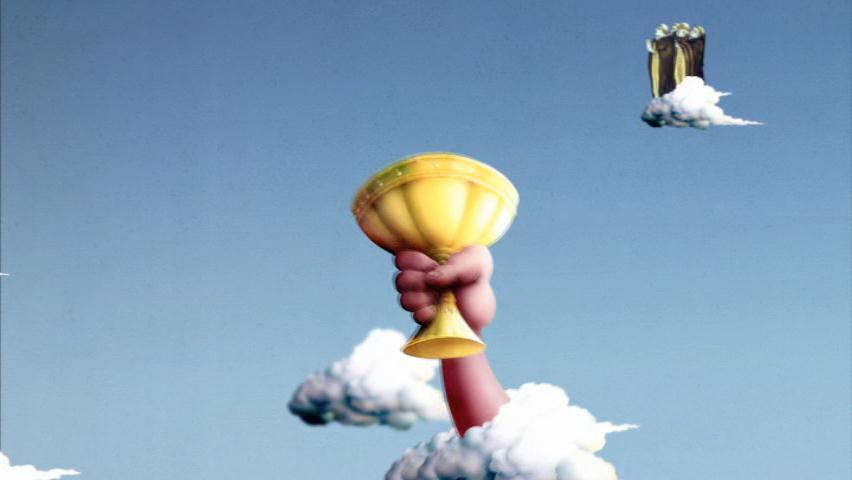
\includegraphics[width=0.8\textwidth]{grail.jpg}
%  \caption[Voorbeeld figuur.]{\label{fig:grail}Voorbeeld van invoegen van een figuur. Zorg altijd voor een uitgebreid bijschrift dat de figuur volledig beschrijft zonder in de tekst te moeten gaan zoeken. Vergeet ook je bronvermelding niet!}
%\end{figure}
%
%\begin{listing}
%  \begin{minted}{python}
%    import pandas as pd
%    import seaborn as sns
%
%    penguins = sns.load_dataset('penguins')
%    sns.relplot(data=penguins, x="flipper_length_mm", y="bill_length_mm", hue="species")
%  \end{minted}
%  \caption[Voorbeeld codefragment]{Voorbeeld van het invoegen van een codefragment.}
%\end{listing}
%
%\lipsum[7-20]
%
%\begin{table}
%  \centering
%  \begin{tabular}{lcr}
%    \toprule
%    \textbf{Kolom 1} & \textbf{Kolom 2} & \textbf{Kolom 3} \\
%    $\alpha$         & $\beta$          & $\gamma$         \\
%    \midrule
%    A                & 10.230           & a                \\
%    B                & 45.678           & b                \\
%    C                & 99.987           & c                \\
%    \bottomrule
%  \end{tabular}
%  \caption[Voorbeeld tabel]{\label{tab:example}Voorbeeld van een tabel.}
%\end{table}

% Inleiding

Hier komt een inleiding...


% Deel 1 - stress en burn-out bij twintigers

\section{Stress en burn-out bij twintigers}
\label{sec:burnout-bij-twintigers}

\subsection{Wat is een burn-out?}
\label{subsec:wat-is-burnout}

\vspace{1em}

Hoewel de term \textit{burn-out} in het dagelijkse taalgebruik steeds frequenter voorkomt, bestaat er vaak onduidelijkheid over de precieze betekenis en afbakening ervan. Een concrete definiëring is dan ook noodzakelijk om het begrip binnen dit onderzoek correct te situeren.

\vspace{1em}

Volgens de elfde herziening van de \acrlong{icd} (\acrshort{icd}-11) van de \acrshort{who} wordt burn-out sinds 2019 omschreven als een syndroom dat het gevolg is van chronische werk gerelateerde stress die onvoldoende werd aangepakt \autocite{world-health-organization-who-2019}. Hoewel het begrip werd opgenomen in de \acrshort{icd}, wordt het niet geclassificeerd als een medische aandoening, maar als een werkgerelateerd fenomeen.

\vspace{1em}

Dit beroepsgerelateerd syndroom wordt gekenmerkt door drie kerncomponenten:
\begin{itemize}
    \item \textbf{Uitputting}: een aanhoudend gevoel van vermoeidheid of mentale uitputting;
    \item \textbf{Cynisme}: een toenemende mentale afstand tot het werk, of een negatieve en cynische houding tegenover de functie;
    \item \textbf{Verminderd gevoel van effectiviteit}: een verminderd gevoel van bekwaamheid en effectiviteit in het uitvoeren van professioneel werk.
\end{itemize}

\vspace{1em}

Ook \textcite{MonteroMarin2011} omschreven burn-out reeds als een syndroom ten gevolge van chronische werkstress, gekenmerkt door uitputting, cynisme en verminderde professionele effectiviteit. Zij benadrukken dat burn-out niet bij iedereen op dezelfde manier tot uiting komt en onderscheiden drie subtypen: \textit{“frenetic”}, \textit{“underchallenged”} en \textit{“worn-out”}.

\vspace{1em}

\subsubsection{Frenetic burnout}
\label{subsubsec:frenetic}

Een hectische burn-out wordt door \textcite{MonteroMarin2011} beschreven als gekenmerkt door passie, ambitie en een sterke betrokkenheid, waarbij personen veel tijd en energie in hun werk steken. Dit kan leiden tot gevoelens van overbelasting en uiteindelijk tot uitputting.

\vspace{1em}

\subsubsection{Underchallenged burnout}
\label{subsubsec:underchallenged}

Bij dit type burnout, aldus \textcite{MonteroMarin2011}, ervaren personen te weinig uitdaging of persoonlijke ontwikkeling in hun werk. Dit gaat vaak gepaard met verveling en onverschilligheid, wat kan resulteren in cynisme. Daarnaast kan de oppervlakkige of repetitieve uitvoering van taken leiden tot een verminderd gevoel van effectiviteit.

\vspace{1em}

\subsubsection{Worn-out burnout}
\label{subsubsec:worn-out}

Wanneer personen het gevoel hebben weinig controle over hun werkzaamheden te hebben en onvoldoende erkenning krijgen voor hun inspanningen, ontstaat het laatste subtype, zoals beschreven door \textcite{MonteroMarin2011}. Dit kan leiden tot passief gedrag, een verminderd gevoel van effectiviteit, versterkt cynisme en bijdragen aan mentale uitputting, vooral door aanhoudende stress en gevoelens van machteloosheid.

\vspace{1em}



\subsection{De huidige burn-out cijfers onder de loep}
\label{subsec:burnout-cijfers}

\vspace{1em}

Recente cijfers van het \textcite{RIZIV2023_invaliditeit_burnout} tonen aan dat burn-out steeds vaker voorkomt in onze samenleving. Eind 2023 werden maar liefst \textbf{45.771} personen gerapporteerd als langdurig arbeidsongeschikt door burn-out, een stijging van bijna 71\% ten opzichte van 26.835 gevallen in 2018. Binnen deze algemene stijging valt vooral de jongste leeftijdscategorie op. Het aantal burn-outgevallen bij volwassenen onder de 30 jaar verdubbelde van 825 in 2018 naar 1.707 in 2023, een \textbf{toename} van \textbf{107\%}, wat de maatschappelijke relevantie van burn-out onder twintigers extra benadrukt \autocite{RIZIV2023_invaliditeit_burnout}.

\begin{figure}[H]
    \centering
    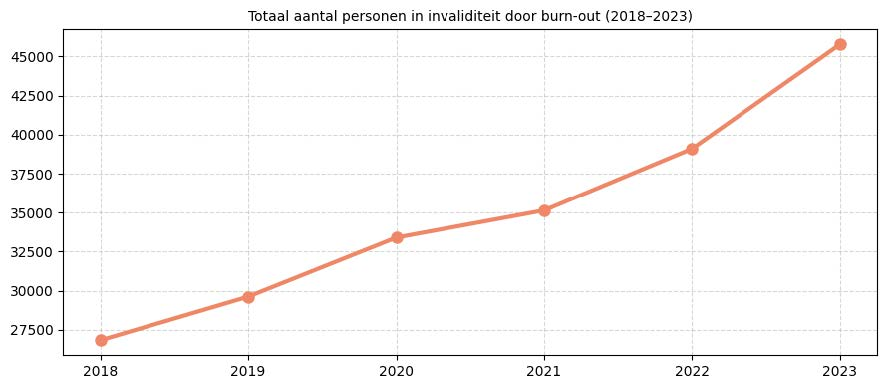
\includegraphics[width=\textwidth]{../graphics/burnout-cijfers-2}
    \caption{Totale evolutie van het aantal personen in invaliditeit door burn-out in België tussen 2018 en 2023 (bron: \autocite{RIZIV2023_invaliditeit_burnout}).}
\end{figure}

\vspace{1em}

\begin{figure}[H]
    \centering
    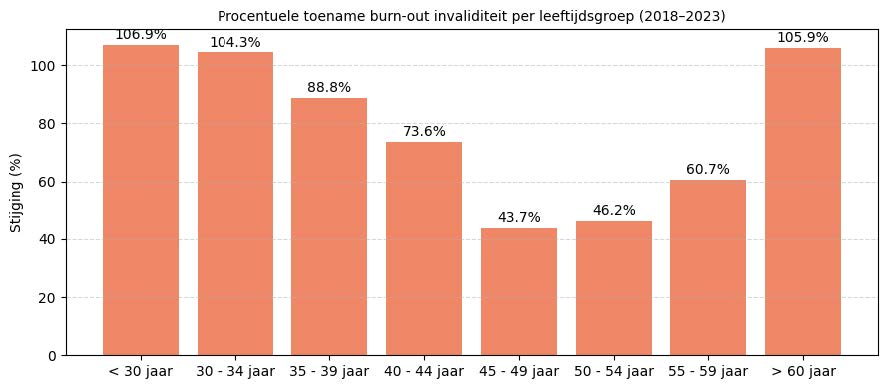
\includegraphics[width=\textwidth]{../graphics/burnout-cijfers-1}
    \caption{\label{fig:procent-stijging-burnout}Procentuele toename van burn-out gerelateerde invaliditeit per leeftijdsgroep tussen 2018 en 2023. Deze verticale staafdiagram maakt duidelijk welke leeftijdsgroepen relatief het sterkst gestegen zijn, met name de groep <30 jaar (bron: \autocite{RIZIV2023_invaliditeit_burnout}).}
\end{figure}

\vspace{1em}
\vspace{1em}
\vspace{1em}
\vspace{1em}

\textcite{SERV2024_werkbaarwerk} bevestigt via hun Vlaamse Werkbaarheidsmonitor daarbij de omvang van het probleem: maar liefst \textbf{13\%} van de jonge werknemers (18-35 jaar) rapporteert symptomen van burn-out, terwijl 35,9\% werkstressklachten ervaart. Dit toont aan dat naast langdurige arbeidsongeschiktheid, ook beginnende burn-outklachten aanzienlijk aanwezig zijn bij jonge werknemers.



\subsection{Kenmerken van de doelgroep}
\label{subsec:kenmerken-generatieZ}

\vspace{1em}

Burn-out is een begrip dat leeft binnen tal van leeftijdscategorieën. In dit onderzoek ligt de focus echter op de groep jonge volwassenen, aangezien uit de voorgaande sectie “Huidige burn-out cijfers onder de loep” blijkt dat bij hen de burn-outcijfers het sterkst stijgen. Om zo specifiek mogelijk te werk te gaan, wordt de doelgroep herleid tot één generatie: \textbf{generatie Z}.

\vspace{1em}

Voordat we ingaan op de risicofactoren die deze generatie kwetsbaar maken voor burn-out, is het eerst essentieel om de kenmerken van generatie Z in kaart te brengen. Dit zowel op het vlak van normen, waarden als van hun gedrag en houding op de werkvloer. 

\vspace{1em}

\subsubsection{Demografische en algemene kenmerken}
\label{subsubsec:demografic-z}

\vspace{1em}

Generatie Z, ook wel gen Z genoemd, is een verzameling aan individuen die geboren zijn tussen 1995 en 2012 \autocite{annerixt-2025}. Het grootste kenmerk aan deze groep, ook wel 14-31 jarigen, is dat ze opgegroeid zijn in een volledig digitale, verbonden wereld waardoor ze al vaak omschreven worden als \textbf{“digital natives”} \autocite{Peredy2024}. Zo zijn ze volgens \textcite{Peredy2024} technisch zeer vaardig, gebruiken ze intensief digitale tools (\textit{zoals sociale media}) en communiceren ze vaak via visuele middelen (\textit{zoals GIFs, memes en korte video’s}). Daarnaast staat deze generatie bekend om haar zeer inclusieve en diverse mindset, sterke maatschappelijke betrokkenheid en ondernemingszin \autocite{Peredy2024}.

\vspace{1em}

\subsubsection{Persoonlijkheidskenmerken}
\label{subsubsec:perskenmerken-z}

\vspace{1em}

Volgens \textcite{annerixt-2025} wordt deze generatie gekenmerkt door een opvallende combinatie van ambitie, perfectionisme, creativiteit en een sterke werkethiek. Ze streven ernaar om uit te blinken in wat ze doen en leggen daarbij veel nadruk op kwaliteit en persoonlijke prestaties. Tegelijkertijd hechten ze veel waarde aan zelfexpressie en persoonlijke ontwikkeling, wat hun verlangen naar autonomie en het vormen van hun eigen identiteit benadrukt \autocite{Zahra2025}.

\vspace{1em}

Ondanks deze sterkte kanten vertoont deze groep ook zwakkere en soms tegenstrijdige eigenschappen. Zo kunnen ze kwetsbaar, zelfgericht en gevoelig voor stress zijn \autocite{annerixt-2025}. Deze combinatie van hoge ambitie en kwetsbaarheid maakt volgens \textcite{Zahra2025} dat individuele erkenning van hun prestaties voor hen van groot belang is.

\vspace{1em}

Samengevat vormt deze generatie een mix van gedrevenheid en creativiteit, gecombineerd met een opvallende gevoeligheid, waarbij persoonlijke ontwikkeling en erkenning centraal staan in hun dagelijks handelen en keuzes.

\vspace{1em}

\subsubsection{Psychologische basisbehoeften op de werkvloer}
\label{subsubsec:psychbehoeften-z}

\vspace{1em}

Steeds meer individuen van generatie Z betreden de werkvloer. Het wordt alsmaar duidelijker dat deze generatie bepaalde psychologische basisbehoeften heeft ontwikkeld die hun functioneren en welzijn sterk beïnvloeden. Volgens \textcite{annerixt-2025} zijn drie kernbehoeften hierbij essentieel: autonomie, competentie en verbondenheid.

\begin{itemize}
    \item \textbf{Autonomie}: het vermogen om zelf keuzes te kunnen maken en controle te hebben over de toegewezen taken;
    \item \textbf{Competentie}: het ervaren van succes en effectiviteit op het werk;
    \item \textbf{Verbondenheid}: ondanks een zekere neiging tot zelfgerichtheid blijft samenwerking, sociale steun en erkenning binnen hun netwerk van groot belang.
\end{itemize}

\vspace{1em}

Naast deze basisbehoeften toont generatie Z een duidelijke focus op mentaal welzijn \autocite{annerixt-2025}. Factoren zoals een gezonde werk-privé balans, erkenning, flexibiliteit en mogelijkheden voor persoonlijke groei zijn voor hen cruciaal. Wanneer deze behoeften onvoldoende vervuld worden, kan dit leiden tot een verhoogd risico op stress, futloosheid en zelfs burn-out \autocite{Zahra2025}. Dit benadrukt dat organisaties die generatie Z optimaal willen ondersteunen niet alleen moeten inzetten op prestaties, maar ook op een omgeving die persoonlijke ontwikkeling en welzijn actief stimuleert.

\vspace{1em}

\subsubsection{Werkhouding, verwachtingen en stressfactoren}
\label{subsubsec:werkhouding-z}

\vspace{1em}

Volgens \textcite{Zahra2025} streeft generatie Z naar zinvol werk, flexibiliteit en mogelijkheden voor persoonlijke groei. Ze willen niet enkel functioneren als “tandwieltjes” in een organisatie, maar vinden het belangrijk dat hun werk bijdraagt aan een groter doel en dat ze zich continu kunnen ontwikkelen.

\vspace{1em}

Echter, door hun ambitieus en perfectionistisch karakter, worden ze regelmatig geconfronteerd met hoge prestatiedruk. De constante blootstelling aan digitale informatie en sociale media zorgt ervoor dat velen zich bijna continu “aan” voelen staan, waardoor het moeilijk is om te ontspannen en echt los te koppelen van werk en verplichtingen \autocite{annerixt-2025}. Bovendien maakt deze generatie zich constant zorgen over hun toekomst, carrièrekansen, financiële situatie, gezondheid, het klimaat en politieke ontwikkelingen, wat bijdraagt aan verhoogde stressniveaus \autocite{annerixt-2025}. 

\vspace{1em}

Hoewel hun technologische vaardigheden de productiviteit en efficiëntie kunnen verhogen, kan overmatig gebruik van digitale tools en sociale media juist leiden tot mentale overbelasting en extra stress \autocite{Zahra2025}. Dit maakt duidelijk dat generatie Z niet alleen behoefte heeft aan uitdagend en betekenisvol werk, maar ook aan een werkomgeving die hen ondersteunt bij het reguleren van werkdruk en het behouden van hun mentale welzijn.

\vspace{1em}



\subsection{Specifieke risicofactoren bij generatie Z}
\label{subsec:risicofactoren-twintigers}



% Deel 2 - digitalisering en cognitieve belasting

\section{Digitalisering en cognitieve belasting}
\label{sec:digitalisering-cognitief}

\subsection{De impact van digitalisering op mentale gezondheid}
\label{subsec:impact-digitalisering}

\subsection{Information overload en permanente bereikbaarheid}
\label{subsec:info-overload}

\subsection{Technostress}
\label{subsec:technostress}

\subsection{Online vigilance}
\label{subsec:online-vigilance}

% Deel 3 - Preventie- en behandelingsstrategieën bij stress en burn-out

\section{Preventie- en behandelingsstrategieën bij stress en burn-out}
\label{sec:preventie-behandeling}

\subsection{Primaire, secundaire en tertiaire preventie}
\label{subsec:preventie-types}

\subsection{Cognitieve-gedragstherapie}
\label{subsec:cgt}

\subsubsection{Rational Emotive Behavior Therapy}
\label{subsubsec:rebt}

\subsubsection{Cognitieve gedragstherapie (CGT)}
\label{subsubsec:cgt-therapie}

\subsection{Psycho-educatie}
\label{subsec:psycho-educatie}

\subsection{Mindfulness}
\label{subsec:mindfulness}

% Deel 4 - Digitale interventies voor mentale gezondheid

\section{Digitale interventies voor mentale gezondheid}
\label{sec:digitale-interventies}

\subsection{E-health en m-health toepassingen}
\label{subsec:e-m-health}

\subsection{Effectiviteit van mentale gezondheidsapps}
\label{subsec:effectiviteit-apps}

\subsection{Engagement en retentieproblematiek}
\label{subsec:engagement-retentie}

\subsection{Kritieken op bestaande mentale gezondheidsapps}
\label{subsec:kritieken-apps}

% Deel 5 - UX- en ontwerpprincipes voor mentale rust

\section{UX- en ontwerpprincipes voor mentale rust}
\label{sec:ux-ontwerp}

\subsection{UI-elementen en cognitieve belasting}
\label{subsec:ui-cognitieve-belasting}

\subsection{Calm design en minimalisme}
\label{subsec:calm-design}

\subsection{Personalisatie en autonomie}
\label{subsec:personalisatie-autonomie}

\subsection{Gamification: ondersteunend of stresserend?}
\label{subsec:gamification}

\subsection{Notificatiestrategieën}
\label{subsec:notificaties}

% Deel 6 - Technologieselectie

\section{Technologieselectie}
\label{sec:technologieselectie}

%%=============================================================================
%% Methodologie
%%=============================================================================

\chapter{\IfLanguageName{dutch}{Methodologie}{Methodology}}%
\label{ch:methodologie}

Om het onderzoek zo succesvol mogelijk te laten verlopen, werd ervoor gekozen het op te splitsen in zes fasen. De eerste fase is een probleemverkenning, waarin een literatuurstudie wordt uitgevoerd om meer inzicht te krijgen in het probleemdomein. Vervolgens wordt een requirements-analyse uitgevoerd, resulterend in een lijst van beoordelingscriteria. Na de requirements-analyse volgt een inventarisatie van het huidige digitale (of analoge) aanbod van burn-outbestrijdingsproduct- en, de zogenaamde longlist-fase. Eenmaal deze producten in kaart zijn gebracht, worden ze teruggebracht tot een shortlist en beoordeeld aan de hand van de eerder opgestelde beoordelingscriteria. Vervolgens is het tijd om de \acrlong{poc} op te stellen. In deze fase worden mock-ups ontwikkeld, de benodigde tools geselecteerd en uiteindelijk een werkend prototype gerealiseerd. Tot slot wordt in de conclusiefase het succes van dit werkende prototype bepaald door middel van een heuristische evaluatie.

\section{Probleemverkenning}
\label{sec:probleemverkenning}

\vspace{1em}

Gedurende de eerste fase is het de bedoeling een diepgaand begrip te krijgen van het probleemdomein aan de hand van een \textbf{literatuurstudie}. Voor dit onderzoek is het essentieel te begrijpen wat een burn-out precies inhoudt, hoe dit speelt bij de huidige generatie twintigers, welke rol digitalisering en een verhoogde cognitieve belasting hierbij kunnen spelen, en welke preventie- en behandelingsstrategieën momenteel beschikbaar zijn. 

\vspace{1em}

Vervolgens wordt het huidige aanbod aan digitale oplossingen voor mentale gezondheid onderzocht, met aandacht voor hun effectiviteit en mogelijke tekortkomingen. Daarbij worden ook UX- en ontwerpprincipes die bijdragen aan mentale rust onder de loep genomen. Tot slot wordt gekeken naar de bestaande technologieën in de app-ontwikkelingswereld, zodat de meest geschikte technologie kan worden geselecteerd voor de ontwikkeling van de proof-of-concept.

\vspace{1em}

Het resultaat van deze fase is een overzicht van de oorzaken van burn-out bij twintigers, hun belangrijkste risicofactoren, en een eerste inventaris van bestaande \newline preventie- en behandelingsstrategieën.

\section{Requirements-analyse}
\label{sec:req-analyse}

\vspace{1em}

Tijdens de requirements-analyse wordt bepaald wat de exacte noden van de doelgroep zijn door middel van het opstellen van functionele en niet-functionele requirements. Deze kunnen enerzijds worden afgeleid uit de reeds verrichte literatuurstudie en anderzijds worden aangevuld door één of meerdere interviews met psychologen. De focus binnen deze studie ligt op het in kaart brengen van effectieve behandelingsmethoden en gebruikerseisen, welke op hun beurt als requirements kunnen worden gedefinieerd.

\vspace{1em}

De requirements worden opgesteld volgens de MoSCoW-methode (Must, Should, Could, Won’t). Deze aanpak maakt het mogelijk om prioriteiten helder te definiëren en de kernfunctionaliteiten concreet te maken. Aan het einde van deze fase ligt er een geprioriteerde lijst van functionele en niet-functionele requirements klaar, die als basis dient voor de \acrlong{poc}.

\section{Longlist}
\label{sec:long-list}

\vspace{1em}

Na de requirements-analyse volgt de inventarisatie van het huidige digitale en analoge aanbod van burn-outbestrijdingsproducten, de longlist-fase. In deze fase worden bestaande alternatieven, zoals apps, websites, wearables en andere concepten, verzameld en geanalyseerd. Alleen oplossingen met een bruikbaar concept dat eventueel digitaal kan worden toegepast, worden opgenomen. De alternatieven worden opgespoord via online bronnen, app-stores en bestaande studies. Elk alternatief wordt vervolgens een eerste keer getoetst aan de opgestelde requirements, zonder dat er al een definitieve beoordeling plaatsvindt. Het resultaat is een overzicht van alle mogelijke alternatieven, inclusief bronvermelding, dat als basis dient voor de volgende fase: de shortlist.

\section{Shortlist}
\label{sec:short-list}

\vspace{1em}

In de shortlist-fase wordt uit de longlist een selectie gemaakt van de meest veelbelovende opties die verder onderzocht zullen worden. Een overzichtelijke matrix ondersteunt de beoordeling van de alternatieven ten opzichte van de gestelde requirements, zodat duidelijk wordt welke oplossingen het beste aansluiten bij de verzamelde criteria en de meest bruikbare componenten bevatten. Aan het einde van deze fase wordt een keuze gemaakt voor één of enkele alternatieven, inclusief de bijbehorende componenten, die meegenomen zullen worden in de ontwikkeling van de \acrlong{poc}.

\section{Proof-of-Concept}
\label{sec:poc}

\vspace{1em}

Tijdens de \acrlong{poc}-fase ligt de focus op het ontwikkelen van een werkend prototype. De ontwikkeling start met het ontwerpen van mock-ups, met speciale aandacht voor mentale rust en minimale cognitieve belasting. Tegelijkertijd wordt bepaald welke app-ontwikkeltechnologie het meest geschikt is. Zodra ontwerp en technologie zijn vastgesteld, volgt de daadwerkelijke uitwerking van het prototype. Dit prototype wordt regelmatig afgetoetst bij de copromotor of andere psychologen om validatie vanuit een professioneel standpunt te waarborgen. Eindgebruikers, met een burn-out of het risico daarop, worden niet betrokken bij deze evaluatie, aangezien zij geen objectief oordeel kunnen geven over de effectiviteit van de oplossing op korte termijn.

\section{Conclusie}
\label{sec:conclusie}

\vspace{1em}

Tot slot, in de conclusiefase, wordt het succes van het werkende prototype beoordeeld aan de hand van een heuristische evaluatie, gebaseerd op de eerder opgestelde evaluatiecriteria en requirements. Deze evaluatie wordt zowel zelfstandig uitgevoerd als door experts, zoals de copromotor, om een professioneel perspectief te waarborgen. Eventuele hiaten of tekortkomingen worden geïdentificeerd, en er worden waar nodig aanbevelingen gedaan voor toekomstig onderzoek. 

\vspace{1em}

Het concrete resultaat van deze fase is een afgeronde analyse van de effectiviteit van de gekozen oplossing, inclusief een overzicht van relevante requirements die ook van waarde kunnen zijn voor andere burn-outgerelateerde IT-projecten. Op deze manier wordt zowel de praktische toepasbaarheid als de wetenschappelijke onderbouwing van het prototype duidelijk gemaakt.

%% TODO: In dit hoofstuk geef je een korte toelichting over hoe je te werk bent
%% gegaan. Verdeel je onderzoek in grote fasen, en licht in elke fase toe wat
%% de doelstelling was, welke deliverables daar uit gekomen zijn, en welke
%% onderzoeksmethoden je daarbij toegepast hebt. Verantwoord waarom je
%% op deze manier te werk gegaan bent.
%% 
%% Voorbeelden van zulke fasen zijn: literatuurstudie, opstellen van een
%% requirements-analyse, opstellen long-list (bij vergelijkende studie),
%% selectie van geschikte tools (bij vergelijkende studie, "short-list"),
%% opzetten testopstelling/PoC, uitvoeren testen en verzamelen
%% van resultaten, analyse van resultaten, ...
%%
%% !!!!! LET OP !!!!!
%%
%% Het is uitdrukkelijk NIET de bedoeling dat je het grootste deel van de corpus
%% van je bachelorproef in dit hoofstuk verwerkt! Dit hoofdstuk is eerder een
%% kort overzicht van je plan van aanpak.
%%
%% Maak voor elke fase (behalve het literatuuronderzoek) een NIEUW HOOFDSTUK aan
%% en geef het een gepaste titel.



% Voeg hier je eigen hoofdstukken toe die de ``corpus'' van je bachelorproef
% vormen. De structuur en titels hangen af van je eigen onderzoek. Je kan bv.
% elke fase in je onderzoek in een apart hoofdstuk bespreken.

%\input{...}
%\input{...}
%...

%%=============================================================================
%% Conclusie
%%=============================================================================

\chapter{Conclusie}%
\label{ch:conclusie}

% TODO: Trek een duidelijke conclusie, in de vorm van een antwoord op de
% onderzoeksvra(a)g(en). Wat was jouw bijdrage aan het onderzoeksdomein en
% hoe biedt dit meerwaarde aan het vakgebied/doelgroep? 
% Reflecteer kritisch over het resultaat. In Engelse teksten wordt deze sectie
% ``Discussion'' genoemd. Had je deze uitkomst verwacht? Zijn er zaken die nog
% niet duidelijk zijn?
% Heeft het onderzoek geleid tot nieuwe vragen die uitnodigen tot verder 
%onderzoek?

Dit onderzoek had als doel na te gaan hoe apps voor stress- en burn-outpreventie het mentale welzijn van Vlaamse twintigers kunnen ondersteunen en hoe inzichten uit bestaande toepassingen kunnen worden vertaald naar concrete ontwerpprincipes en functionaliteiten voor een \acrshort{poc}. Op basis van de literatuurstudie, het expertinterview, de requirementsanalyse, de analyse van bestaande toepassingen en de ontwikkeling en evaluatie van de \acrshort{poc} kunnen de onderzoeksvragen als volgt worden beantwoord.

\vspace{1em}

\section{Het probleem}
\label{sec:het-probleem-conclusie}

\vspace{1em}

Vlaamse twintigers vormen geen homogene doelgroep en hebben bijgevolg ook niet allemaal dezelfde noden op vlak van mentale gezondheid. Binnen generatie Z kan voornamelijk een onderscheid worden gemaakt tussen studenten en jongvolwassenen die actief zijn op de arbeidsmarkt. Studenten ervaren onder meer academische verwachtingen en prestatiedruk, terwijl werkende twintigers bijkomende druk kunnen ervaren door werkbelasting, loopbaanverwachtingen en financiële onzekerheid. Tegelijkertijd zijn er verschillende gedeelde kenmerken, zoals perfectionisme, ambitie, sociale vergelijking en een sterke behoefte aan erkenning en persoonlijke ontwikkeling. Vooral de psychologische basisbehoeften aan autonomie, competentie en verbondenheid zijn hierbij relevant. Een ondersteunende toepassing moet daarom voldoende flexibel zijn om rekening te houden met verschillende levenssituaties, terwijl ze tegelijkertijd deze gedeelde behoeften ondersteunt.

\newpage

De manier waarop deze persoonlijke en externe factoren worden ervaren, heeft ook invloed op de gebruikerservaring van digitale toepassingen. Werk-, studie- en sociale druk kunnen ervoor zorgen dat gebruikers reeds met een hoge mentale belasting een toepassing openen. Een hoge mate van digitale connectiviteit, voortdurende bereikbaarheid en sociale vergelijking kunnen deze belasting verder versterken door information overload, technostress en een verhoogde alertheid voor digitale prikkels. Een toepassing die mentale ondersteuning wil bieden, moet daarom vermijden dat ze zelf bijkomende inspanning vraagt. Duidelijke visuele hiërarchie, beperkte informatie per scherm, korte teksten, eenvoudige navigatie en het opdelen van complexe informatie in kleinere stappen zijn hierdoor belangrijke voorwaarden voor een ondersteunende gebruikerservaring.

\vspace{1em}

Het bestaande aanbod voor mentale gezondheid biedt hiervoor nog geen volledige oplossing. Mentale gezondheidsapps richten zich voornamelijk op mindfulness, meditatie en ademhalingsoefeningen, terwijl andere interventievormen, zoals \acrshort{rebt}, minder vertegenwoordigd zijn. Ook toepassingen die specifiek gericht zijn op burn-outpreventie blijken schaars en er is weinig sprake van één geïntegreerde toepassing die verschillende preventieve interventies combineert. Daarnaast kunnen complexe navigatie, beperkte personalisatie, overvolle interfaces, onduidelijke communicatie en een grote hoeveelheid notificaties de cognitieve belasting verhogen. Het falen van bestaande toepassingen ligt daardoor niet noodzakelijk in een gebrek aan inhoudelijke interventies, maar vooral in de combinatie van inhoud, gebruikerservaring en de context waarin deze wordt aangeboden.

\vspace{1em}

Binnen de bestaande apps voor mentaal welzijn worden voornamelijk mindfulness, meditatie, ademhalingsoefeningen, dagboeken, stemmingsregistratie en psycho-educatie toegepast. Deze functionaliteiten kunnen waardevol zijn, maar hun meerwaarde wordt mede bepaald door de manier waarop ze worden aangeboden. De analyse wijst daarom op het belang van aanvullende principes zoals personalisatie, autonomie, overzichtelijkheid, beperkte digitale prikkels en ondersteuning van persoonlijke vooruitgang. Een goede mentale gezondheidsapp hoeft bijgevolg niet zoveel mogelijk functionaliteiten te bevatten, maar moet vooral de juiste functionaliteiten op een samenhangende en laagdrempelige manier aanbieden.

\vspace{1em}


\section{Functionele en niet-functionele vereisten}
\label{sec:requirements-conclusie}

\vspace{1em}

Voor een toepassing die stress en burn-out bij twintigers helpt voorkomen, zijn zowel inhoudelijke functionaliteiten als kwaliteitsvoorwaarden essentieel. Tot de belangrijkste functionaliteiten behoren onboarding en personalisatie, stressregistratie en zelfreflectie, een gestructureerd dagboek met historiek, psycho-educatie, stressreducerende oefeningen, feedback en zichtbare persoonlijke vooruitgang. 

Ook instelbare notificaties en mogelijkheden tot ondersteuning en doorverwijzing naar professionele hulp zijn relevant. Deze functionaliteiten moeten worden aangeboden binnen kwaliteitsvoorwaarden zoals bruikbaarheid, toegankelijkheid, performantie, betrouwbaarheid, beveiliging en privacy. Zeker bij gevoelige mentale gezondheidsinformatie moeten gebruikers controle behouden over hun gegevens en over de manier waarop zij met de toepassing interageren.

\vspace{1em}


\section{UI/UX en mentale rust}
\label{sec:UI-UX-mentale-rust}

\vspace{1em}

Een rustige gebruikerservaring ontstaat vooral door informatie en prikkels bewust te beperken. Overzichtelijkheid, een duidelijke visuele hiërarchie, consistente interacties, beperkte informatie per scherm en eenvoudige navigatie dragen bij aan mentale rust. Ook chunking, progressive disclosure, korte scanbare teksten en één primaire taak per scherm beperken de hoeveelheid informatie die gebruikers tegelijk moeten verwerken. Een rustig kleurenpalet, beperkt gebruik van fonts en kleuren, weinig animaties en terughoudend gebruik van afbeeldingen en video helpen daarnaast visuele overprikkeling te voorkomen. Complexe navigatie, overvolle interfaces, inconsistente interacties en grote hoeveelheden informatie werken daarentegen in de tegenovergestelde richting en verhogen de cognitieve belasting.

\vspace{1em}

Deze inzichten kunnen worden vertaald naar concrete ontwerpprincipes voor een interface die mentale rust bevordert. Daarbij staan onder meer privacy by design, inclusieve toegankelijkheid, beperkte digitale interrupties, behoud van overzicht, minimalisering van cognitieve belasting, het vermijden van visuele overprikkeling en techno-simplicity centraal. Daarnaast moeten ontwerpkeuzes autonomie, competentie, verbondenheid, persoonlijke relevantie en betekenisvolle vooruitgang ondersteunen. De interface moet de gebruiker dus niet alleen informeren of activeren, maar vooral het gevoel geven dat de toepassing ondersteunend, beheersbaar en relevant is.

\vspace{1em}

Ook notificaties en gamification vragen om een terughoudende aanpak. Meldingen kunnen helpen bij gedragsverandering en engagement, maar kunnen tegelijkertijd digitale overbelasting en online vigilance versterken. Ze moeten daarom optioneel, instelbaar, beperkt, contextafhankelijk en gepersonaliseerd zijn en mogen niet dwingend of urgent worden geformuleerd. Gamification kan eveneens ondersteuning bieden, zolang de nadruk ligt op persoonlijke groei en betekenisvolle vooruitgang. Punten, rankings en competitieve streaks zijn minder geschikt omdat ze de focus kunnen verschuiven van welzijn naar prestatie. Spelelementen moeten bijgevolg het gezondheidsdoel ondersteunen en geen nieuwe prestatiedruk creëren.

\vspace{1em}


\section{Beantwoording van de hoofdonderzoeksvraag}
\label{sec:beantwoording-hoofdonderzoeksvraag}

\vspace{1em}

Apps voor stress- en burn-outpreventie kunnen het mentale welzijn van Vlaamse twintigers ondersteunen wanneer inhoudelijke interventies worden gecombineerd met een gebruikerservaring die zelf geen bijkomende bron van stress vormt. De resultaten tonen aan dat hiervoor niet alleen relevante functionaliteiten nodig zijn, maar ook een sterke focus op personalisatie, autonomie, overzichtelijkheid, beperkte digitale prikkels en cognitieve rust. De opgestelde requirements en ontwerpprincipes bieden hiervoor een concreet kader, terwijl de \acrshort{poc} aantoont dat deze inzichten kunnen worden vertaald naar concrete ontwerp- en ontwikkelkeuzes. De meerwaarde ligt daarmee niet in het aanbieden van zoveel mogelijk functies, maar in het doelgericht combineren van functionaliteit, interface en interactie zodat de toepassing ondersteunt zonder bijkomende cognitieve belasting of prestatiedruk te veroorzaken.

\vspace{1em}

De resultaten liggen grotendeels in lijn met de verwachtingen uit het oorspronkelijke onderzoeksvoorstel. Zo werd bevestigd dat mindfulness, meditatie en ademhalingsoefeningen sterk vertegenwoordigd zijn in bestaande toepassingen, terwijl andere interventievormen minder vaak voorkomen. Ook kwamen verschillende potentiële bronnen van cognitieve belasting, zoals complexe navigatie, grote hoeveelheden informatie en frequente notificaties, terug in de analyse. Dit bevestigt dat niet alleen de inhoud van een mentale gezondheidsapp, maar ook de manier waarop deze wordt aangeboden, bepalend is voor de potentiële meerwaarde ervan.

\vspace{1em}


\section{Beperkingen}
\label{sec:beperkingen}

\vspace{1em}

Hoewel deze bachelorproef een onderbouwde ontwerpaanpak en \acrlong{poc} heeft opgeleverd, zijn er verschillende beperkingen. De belangrijkste beperking is dat de ontwikkelde \acrshort{poc} niet werd geëvalueerd met eindgebruikers. De evaluatie gebeurde voornamelijk aan de hand van een heuristische beoordeling van de requirements en ontwerpprincipes, aangevuld met een evaluatie door de copromotor. Hierdoor kon worden nagegaan in welke mate de voorgestelde ontwerpkeuzes werden toegepast, maar niet of gebruikers deze daadwerkelijk als rustgevend, begrijpelijk of ondersteunend ervaren. De resultaten tonen daarom vooral aan dat de voorgestelde ontwerpaanpak praktisch toepasbaar is en vormen geen bewijs dat de toepassing daadwerkelijk stress- of burn-outklachten vermindert.

\vspace{1em}

Een tweede beperking betreft de concretisering van de ontwerpprincipes. Het principe rond inclusieve toegankelijkheid is bijvoorbeeld relatief breed geformuleerd en verwijst naar de \acrshort{wcag}-richtlijnen, die een omvangrijk geheel aan criteria bevatten. Binnen de scope van deze bachelorproef was het niet haalbaar om deze volledig te vertalen naar concrete en controleerbare criteria. Daarnaast werden de ontwerpprincipes door de onderzoeker zelf toegepast. De aanwezige voorkennis uit de opleiding grafisch ontwerp en de verdieping in het onderzoeksdomein kunnen daardoor invloed hebben gehad op de interpretatie en toepassing ervan. Het is bijgevolg nog niet duidelijk in welke mate andere ontwerpers of ontwikkelaars dezelfde principes op een gelijkaardige manier zouden interpreteren.

\vspace{1em}

Ten slotte is de toepasbaarheid van de ontwerpprincipes buiten het domein van mentale gezondheidsapps nog onvoldoende onderzocht. Hoewel verschillende principes, zoals het beperken van cognitieve belasting, het ondersteunen van autonomie en het vermijden van prestatiedruk, mogelijk ook relevant zijn voor andere digitale toepassingen, werd dit binnen deze bachelorproef niet onderzocht.

\vspace{1em}

\section{Aanbevelingen voor verder onderzoek}
\label{sec:verder-onderzoek}

\vspace{1em}

Een eerste belangrijke stap voor verder onderzoek is een evaluatie met eindgebruikers. Een gebruikerstest en, bij voorkeur, een langdurige evaluatie kunnen nagaan of gebruikers de toepassing daadwerkelijk als minder cognitief belastend ervaren en of de ontwerpkeuzes op langere termijn samenhangen met veranderingen in ervaren stress. Hierbij kan zowel worden onderzocht of gebruikers de functionaliteiten begrijpen en waarderen als of de ontwerpprincipes daadwerkelijk bijdragen aan een ondersteunende gebruikerservaring.

\vspace{1em}

Daarnaast is verder onderzoek nodig naar de overdraagbaarheid en reproduceerbaarheid van de ontwerpprincipes. Omdat de principes binnen deze bachelorproef door de onderzoeker zelf werden toegepast, kan toekomstig onderzoek waarbij externe ontwerpers of developers de richtlijnen toepassen inzicht geven in de mate waarin deze voldoende concreet en eenduidig zijn. Dit kan bovendien aantonen welke principes verdere concretisering nodig hebben.

\vspace{1em}

Tot slot kan worden onderzocht in welke mate de ontwerpprincipes toepasbaar zijn buiten mentale gezondheidsapps. Principes zoals het beperken van cognitieve belasting, het vermijden van prestatiedruk, het respecteren van rustmomenten en het ondersteunen van autonomie zijn niet noodzakelijk gebonden aan mentale gezondheid. Het kan daarom waardevol zijn om na te gaan of dezelfde ontwerpaanpak ook kan bijdragen aan een minder belastende gebruikerservaring binnen bijvoorbeeld sociale media, productiviteitsapplicaties of andere digitale toepassingen waarin gebruikers grote hoeveelheden informatie en taken moeten verwerken.

%---------- Bijlagen -----------------------------------------------------------

\appendix

\chapter{Onderzoeksvoorstel}

Het onderwerp van deze bachelorproef is gebaseerd op een onderzoeksvoorstel dat vooraf werd beoordeeld door de promotor. Dat voorstel is opgenomen in deze bijlage.

\section*{Samenvatting}

De afgelopen jaren stijgt het aantal burn-outs bij jongvolwassenen aanzienlijk, mede door de druk van de quarter-life-crisis en digitale overbelasting. Hoewel er steeds meer apps bestaan om mentaal welzijn te ondersteunen, blijkt hun effect beperkt en verhogen sommige toepassingen juist cognitieve belasting. Deze bachelorproef onderzoekt daarom de vraag: \emph{“Hoe kunnen apps voor stress- en burn-out-preventie het mentale welzijn van Vlaamse twintigers verbeteren, door middel van inzichten uit een analyse van bestaande apps te vertalen naar concrete ontwerpprincipes en functionaliteiten voor een proof-of-concept app?”}. Om dit te realiseren wordt een methodologie bestaande uit 6 fasen toegepast: eerst een probleemverkenning via literatuurstudie en interviews met professionals, gevolgd door een gestructureerde requirementsanalyse (MoSCoW), het opstellen van een long- en shortlist van bestaande oplossingen, en de ontwikkeling van een cognitief rustgevende proof-of-concept. Tot slot wordt de effectiviteit van het prototype geëvalueerd via een heuristische beoordeling door professionals. Het verwachte resultaat is een wetenschappelijk onderbouwde app die stress vermindert, mentale rust bevordert en cognitieve belasting minimaliseert, terwijl ze herbruikbare ontwerpprincipes oplevert voor andere digitale toepassingen en zo zorgprofessionals ondersteunt. Hiermee draagt het onderzoek bij aan het mentale welzijn van Vlaamse twintigers en biedt het een concrete meerwaarde voor gebruikers, professionals, en het bredere welzijn van de samenleving.

% Verwijzing naar het bestand met de inhoud van het onderzoeksvoorstel
\input{../voorstel/voorstel-inhoud}

%%---------- Andere bijlagen --------------------------------------------------
% TODO: Voeg hier eventuele andere bijlagen toe. Bv. als je deze BP voor de
% tweede keer indient, een overzicht van de verbeteringen t.o.v. het origineel.
%\input{...}

%%---------- Backmatter, referentielijst ---------------------------------------

\backmatter{}

\setlength\bibitemsep{2pt} %% Add Some space between the bibliograpy entries
\printbibliography[heading=bibintoc]

\end{document}
